The bloc-diagram of the impedance-sensing device constructed for IFC application in this memoir is shown in \autoref{fig:BlocDiagramElectronics}. From a bird's eyes view, it works by sending a programmable signal voltage to the SUT, and then measuring it's current response. It uses square waveform as input instead of the conventional sinewave to reduce the power consumption, as explained in \autoref{sec:PSD}. Thus, a square waveform with frequency ranging from 200kHz to 200MHz is created by the clock-component Si5351 \cite{si5351datasheet}. This square waveform is sent to a quadrature generator (see \autoref{sec:QuadratureGenerator}) to create two 90-degree phase-shifted square waveforms at half the clock-component signal frequency. The in-phase waveform is attenuated and sent to the two diffential electrode pairs of the microfluidics system. Their two current responses are amplified and converted to voltage signals by TIAs \cite{horowitz1989art} (see \autoref{sec:TIA}), then mixed by the two PSDs (see \autoref{sec:PSD}). This yields four output signals that can finally be sampled by the ADCs: the real and imaginary current responses of two electrode pairs. The impedance magnitude and phase can be retrieved numerically in post-processing from the real and imaginary impedance components, after correcting the dataset with a square-to-sine algorithm. \par
\begin{figure}[h]
    \centering
    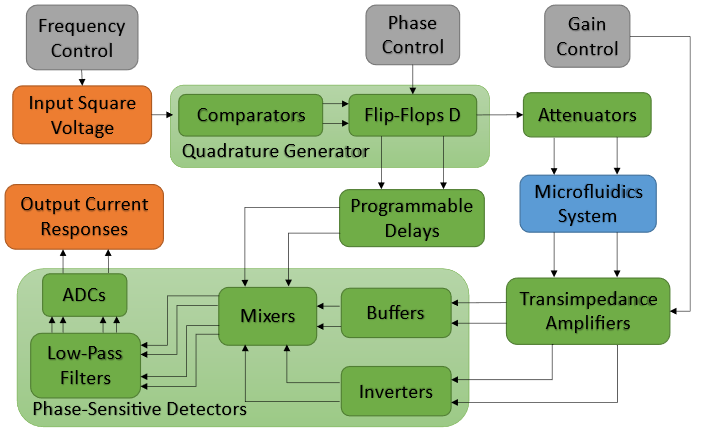
\includegraphics[width=1\textwidth]{BlocDiagramElectronics}
    \caption{Bloc-diagram of the impedance-sensing device constructed in this study.}
    \label{fig:BlocDiagramElectronics}
\end{figure}

Let's describe the methodology in detail from the beginning. \par

The square wave input voltage $V_{in}$ sent to the electrodes is defined in time by \autoref{eq:Squarewave}, as described in \autoref{sub:SquareSignal}. It has a known initial magnitude $V_0$ at the output of the comparator, and is attenuated by a factor $A$ to be at a low enough value of about $~100mV$ for linear impedance measurements that won't harm the cells:
\begin{equation}
   V_{in}(t) = \frac{4}{\pi} \frac{V_0}{A} \displaystyle\sum_{n=1,3,5,7...} ^{\infty} \frac{\sin(n \omega_0 t)}{n}
\end{equation}

This input voltage produces current responses from the two electrode pairs, which follow Ohm's law for complex impedances. This current response being difficult to interact with, two TIAs are used to convert them to voltage signal. Considering the simplified \autoref{eq:TIA_simple} for the transimpedance without $C_f$ and $C_i$, the following equation is obtained:
\begin{equation}
\label{eq:V_TIA}
   V_{TIA}(t) = -\frac{4}{\pi} \frac{V_0}{A} R_f \displaystyle\sum_{n=1,3,5,7...} ^{\infty} \frac{\sin(n \omega_0 t)}{n\lvert Z \rvert (n \omega_0 t + \theta)}
\end{equation}
Where $\lvert Z \rvert (n \omega_0 t + \theta)$ is the impedance magnitude and phase of the SUT at the harmonic frequency $n \omega_0$.  \par

The TIAs current outputs being at high frequency, they cannot be directly sampled by a microcontroller (as already described in \autoref{sec:LIA}). A mixing and filtering stage implemented from a PSD is thus used, which creates DC values proportional to the real and imaginary parts of the current responses (see \autoref{sec:PSD}). These DC values can easily be sampled by ADCs, and follow the equation: \par
\begin{equation}
\label{eq:RealPSD}
   \Re(V_{PSD-\omega_0}) = \frac{1}{2} \frac{6}{\pi^2} \frac{V_0 R_f}{A} \displaystyle\sum_{n=1,3,5,7...} ^{\infty} \frac{\cos(\theta(n \omega_0))}{n^2\lvert Z \rvert (n \omega_0)}
\end{equation}
\begin{equation}
\label{eq:ImPSD}
   \Im(V_{PSD-\omega_0}) = \frac{1}{2} \frac{6}{\pi^2} \frac{V_0 R_f}{A} \displaystyle\sum_{n=1,3,5,7...} ^{\infty} \frac{\sin(\theta(n \omega_0))}{n^2\lvert Z \rvert (n \omega_0)}
\end{equation}
It should be noted that the amplitudes of the reference voltage signal of the PSDs don't influence the previous equations since they are used only to operate the switches. \par 

The real and imaginary outputs of the two PSDs are sampled by four ADCs which have a resolution limit $R_{ADC}$ theoretically fixed by their number of bits, but practically limited by the $ENOB$ (see \autoref{sec:ADC}). This means that a low enough voltage response from the PSDs measured at the ADCs will be undistinguishable from the noise floor. \par

Considering the inverse proportionality of $\lvert Z \rvert$ in \autoref{eq:RealPSD} and \autoref{eq:ImPSD}, the SNR will decrease subtantially as the SUT's impedance increases. To solve this issue, a PGA is added to the system to modify the gain at will (see \autoref{sec:PGA}). This leads to a higher voltage signal at the ADC, which increases the SNR in return. The gain resistor of the PGA should thus always be chosen to maximize the voltage signal, without saturating the ADCs or the op-amps. Indeed, the ADCs and op-amps only operate for voltages in between the power-supplies $V_{DD}$ and $V_{SS}$ (see \autoref{sec:Power-Supplies}). \par

 Now, as can be seen from \autoref{eq:RealPSD} and \autoref{eq:ImPSD}, it isn't trivial to recover the impedance magnitude and phase since harmonics of the square excitation signal are present at every odd frequency of the fundamental \cite{Subhan2019}. Square-waves being used in the mixer instead of sinewaves introduces a systematic error in the impedance measurement. These harmonics are multiplied together by the mixer, which pushes them to DC along with the desired fundamental frequency. Mathematically, this situation adds a geometric sum factor error on the value of impedance measured. This error can be corrected by subtracting the impedance values measured at the harmonics frequencies, as shown in \autoref{fig:SubhanSquare2Sine}. It is thus necessary to measure the entire impedance spectrum before computing the adjusted impedances. \par
\begin{figure}[h]
    \centering
    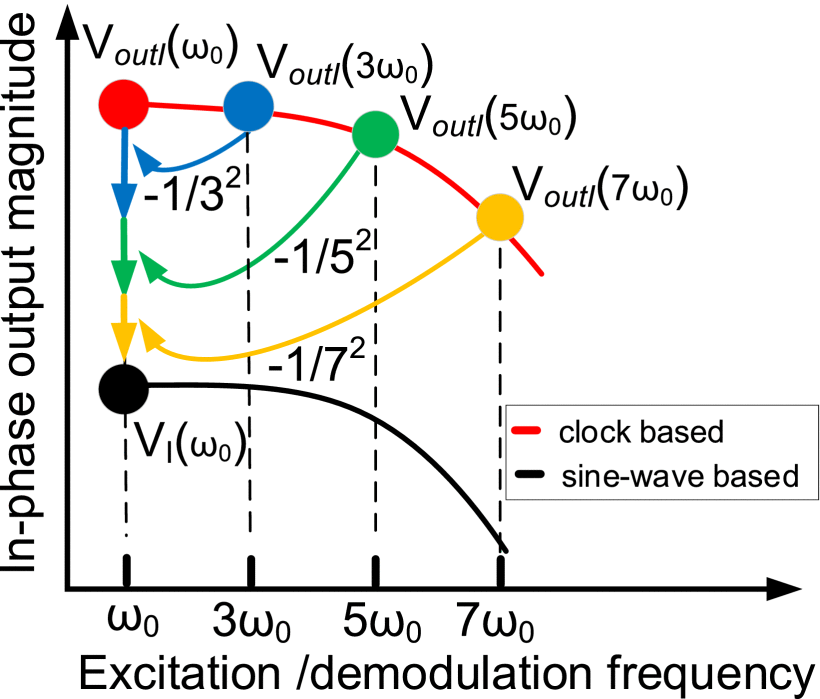
\includegraphics[width=0.7\textwidth]{SubhanSquare2Sine}
    \caption{Illustrated principles of the error-cancellation method proposed by \citep{Subhan2019}.}
    \label{fig:SubhanSquare2Sine}
\end{figure}

This algorithm to convert from a square wave spectroscopy to a sinewave spectroscopy is taken almost directly from \citep{Subhan2019} and modified to fit the system used in this study. The values of square impedances at the harmonics can be subtracted or added to the fundamental impedance following a certain set of rules described in \citep{Subhan2019}. Following these rules, it is possible to retrieve the impedance spectroscopy real and imaginary components devoid of the systematic error $V_{sine-\omega_0}$. This process is described here :  
\begin{align}
\label{eq:correctionReal}
   \Re(V_{sine-\omega_0}) &= \displaystyle\sum_{n=1,3,5,7...} ^{\infty} \frac{\cos(\theta(n \omega_0))}{n^2\lvert Z \rvert (n \omega_0)} - \displaystyle\sum_{n=3,5,7...} ^{\infty} \frac{\cos(\theta(n \omega_0))}{n^2\lvert Z \rvert (n \omega_0)}\nonumber\\
   \Re(V_{sine-\omega_0}) &= \frac{\cos(\theta(\omega_0))}{\lvert Z \rvert (\omega_0)} + E
\end{align}
Where $E$ is the residual error after correction. The same process can be repeated for the quadrature component:
\begin{equation}
   \Im(V_{sine-\omega_0}) = \frac{\sin(\theta(\omega_0))}{\lvert Z \rvert (\omega_0)} + E
\end{equation}
The corrected impedance magnitude and phase can then be reconstructed based on \autoref{eq:Magnitude} and \autoref{eq:Phase}.
\begin{equation}
    \label{eq:CorrectedMagnitude}
   \lvert Z(\omega_0) \rvert = \frac{1}{2} \frac{6}{\pi^2} \frac{V_0}{A} R_f \frac{1}{\sqrt{(\Re(V_{sine-\omega_0}))^2+(\Im(V_{sine-\omega_0}))^2)}}
\end{equation}
\begin{equation}
\label{eq:CorrectedPhase}
   \theta(\omega_0) = -\atan(\frac{\Im(V_{sine-\omega_0})}{\Re(V_{sine-\omega_0})})
\end{equation}